\chapter{Contribution}
\label{chap:contribution}
This chapter explain the contribution of this thesis. \Cref{sec:contributionDingNet} start presenting all the work done to extend and evolve the DingNet simulator, and terminate with a validation scenario. \Cref{sec:contributionACOverDingNet} present the work done to support the execution of aggregate computing program over the DingNet simulator, and in particular Protelis program. 

\section{Extension and evolution to DingNet}
\label{sec:contributionDingNet}
This section presents all the improvement, extension, and evolution applied to the DingNet simulator to achieve an extendible and configurable simulator, that simulates the entire LoRa-over-MQTT network. 
Previous works on the simulator\todo{intro phrase} were focused mainly on three areas:
\begin{enumerate}
    \item \textbf{LoRaWAN communications}: simulation of bi-directional communication between LoRa motes and LoRa gateway
    \item \textbf{GUI}: provide a good user interface that simplify the configuration of simulation and allow the user to see the simulation result
    \item \textbf{Self-adaptive applications}: evaluation of algorithms to reduce the energy consumption for LoRa motes communication, but ensuring that each transmission is received at least from one gateway.
\end{enumerate}
The following part of the section presents the contribution to the DingNet simulator (part of this work was done in collaboration with Federico Quin, a PhD student at KU Leuven).
\clearpage
\subsection{Build tool and Continuous Integration}
After a first study of the simulator's project, it was noticed the absence of a build tool to manage project's dependency, build, and execution, so the first action was been to add it. 
In a first moment was chosen \textit{Apache Maven} as build tool, but then \textit{Gradle} was preferred to it for several reasons\footnote{ \href{https://gradle.org/maven-vs-gradle/}{https://gradle.org/maven-vs-gradle (Feb 2020)}}. The main reasons that guided this change are: performance, highest readability of project's configuration file due to a less verbosity syntax, and better script support (with possibility to write them in kotlin with \textit{Gradle Kotlin DSL}). 

In the context of project management another important aspect is the continuous integration, that is useful to build and test the project in automatic way in different and fresh environment. 
As continuous integration service to test the project in all the main operative systems (linux, windows, and osx) and with different java versions (11 and 12) was chosen \textit{Travis-CI}\footnote{\href{https://travis-ci.com/}{https://travis-ci.com (Feb 2020)}}.
Travis-CI was chosen because it is free and well integrated with \textit{GitHub} that host the project.

\subsection{Code improvement}
Before start to evolve the simulator it was been necessary to carry out a phase for improve the code already present. 
This phase has the aim to improve the readability of the code and apply the KISS principle to prevent possible bug.
The main actions was been: use of base type and base interface instead class type, reduce code duplication reorganizing code or moving it inside method, remove magic number replacing them with constants, avoid to use useless functions, define unit of measure of physical concepts, apply tools for style checking to guarantee code readability over time.

\subsection{Spatial reference system}
The first important intervention involve the spatial reference system (SRS) of the simulation environment. Original SRS was a discrete one and this leads that:
\begin{itemize}
    \item low precision for displacement of gateways and motes in the environment
    \item mobile mote assume a Manhattan movement style to move from a point A to a point B. 
\end{itemize}  
To increase the precision for the displacement of the entities and move mobile motes from point A to B with straight lines it was been necessary to convert the discrete SRS to a continuous one. 

\subsection{Change representation of the time}
Another important intervention involve the representation of the time of simulation. Previously the time was represented by the java class \mbox{\textit{LocalTime}}. This representation has two problems. 
The first problem is that it does not allow to execute simulation with duration of more than one day because it does not include the concept of \textit{day}. 
The second one is that it does not allow direct manipulation of the time based on the unit of measure of millisecond, that it is the mainly unit used inside the simulator.
To solve both the previous problems was introduced an own concept of time. 
This representation of the time, figured in \autoref{fig:time}, allows to manipulate it in a simply way providing different methods for the different units of measure.
\begin{figure}[h]
    \centering
    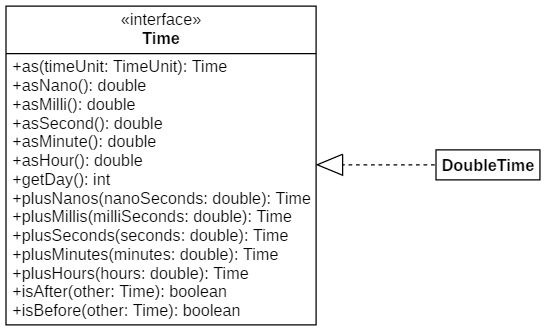
\includegraphics{figures/time.png}
    \caption[Time representation in DingNet simulator]{Time representation that provides all the basic functionality.}
    \label{fig:time}
\end{figure}

% \subsection{Change simulation loop}
% redesing simulation loop using timer event instead loop with time checking,

\subsection{Communication protocol between mote and gateway}
%  communication protocol mote-gateway (interface sender and receiver).
In the LoRaWAN protocol every mote can start a transmission at every time based on its needs, without checks the transmission medium (ALOHA-like protocol).
Actually the simulator implements this behaviour inside the class \mbox{\textit{NetworkEntity}}, that is the base class for \mbox{\textit{Gateway}} and \mbox{\textit{Mote}}. 
To generalize this behaviour and allow to evaluate the network behaviour with several variants of ALOHA-like protocol it is modified the existing architecture with that proposed in \autoref{fig:sendRec}.
\mbox{\textit{Sender}} interface defines methods to send a packet, check the transmission status, and manage parameters that influence the transmission; while the \mbox{\textit{Receiver}} interface defines methods to receive incoming transmissions, and allow to the \mbox{\textit{NetworkEntity}} to specify how to manage them.
\todo{caption to figure}
\begin{figure}[h]
    \centering
    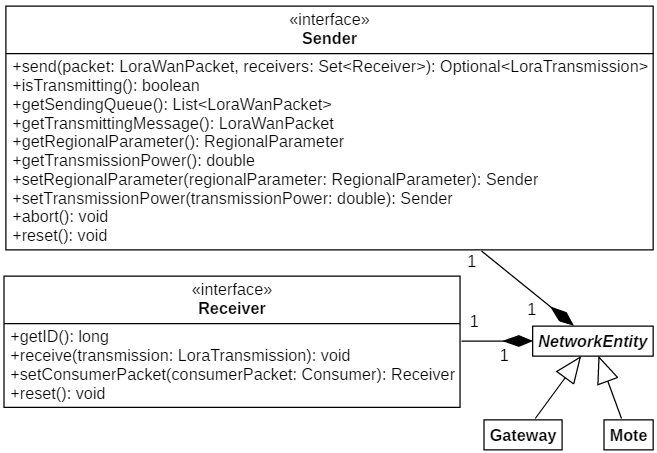
\includegraphics{figures/sendRec.png}
    \caption{}
    \label{fig:sendRec}
\end{figure}

\subsection{Managing of incoming message to a LoRa mote}
The LoRaWAN protocol allows communication from gateways to motes, also if it is discourage for physical limitation of the transmission medium. 
The simulator already support this communication, but it is designed only the structure to manage \textit{MAC Commands} (special commands exchanges between network server and motes for network administration) motes side.
To complete the managing of incoming message to a LoRa mote allowing to use all the information presents in the payload it is designed the architecture presented in \autoref{fig:consume}.
\mbox{\textit{ReceivedPacketStrategy}} define the strategy to use to store all the incoming packets and manage the pending queue of packets to consume.
\mbox{\textit{ConsumePacketStrategy}} define a how use the information in the payload to produce a side-effect on the LoRa mote or in the environment. 
Every mote can have a list of \mbox{\textit{ConsumePacketStrategy}} that are executed in an ordered way with strategy that can use or ignore the packet.
\autoref{fig:consume} shows two implementation for the \mbox{\textit{ReceivedPacketStrategy}}, and none for \mbox{\textit{ConsumePacketStrategy}}, this because the first strategies are cross domain while the second ones are domain specific respect the simulated applications.
\begin{figure}[h]
    \centering
    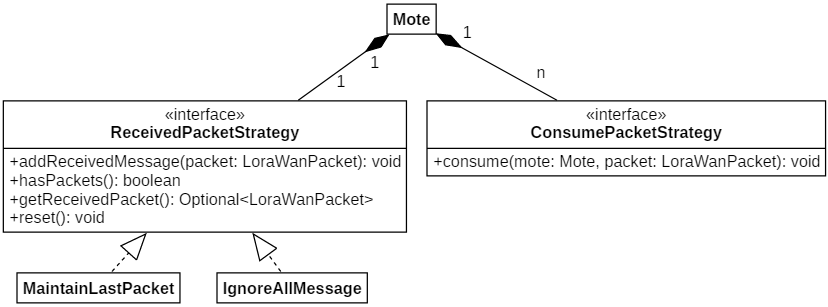
\includegraphics[width=\textwidth]{figures/consumePacket.png}
    \caption{Architecture for manage incoming packets motes side}
    \label{fig:consume}
\end{figure}

\subsection{Communication between Gateways and Applications}
In a LoRa-over-MQTT network, communications between gateways and applications are MQTT based and intermediated by the network server, but actually in the simulator missing both the network server and MQTT communication. 
So to simulate in a batter way the network's behaviour is necessary to implements both.

\subsubsection{MQTT communication}
\todo{rifrasare tutto}
In addition to emulating the MQTT behaviour are defined the following requirements for the MQTT client:
\begin{itemize}
    \item[Req1.] allow to change client implementation in a simple and fast way (for example from a mock implementation to a real one). 
    This requirement is useful to allow simulation with different client abstraction, optimization, and realize a simulator technology independent for MQTT client's implementation
    \item[Req2.] avoid conversion of MQTT message to a domain specific object at each topic \mbox{subscription}.
\end{itemize}
To respect Req1 is necessary to avoid to use directly reference to a particular implementation, so was been defined the interface \mbox{\textit{MqttClient}}.
It represents a MQTT client and provide all the basic functionality to interact with a MQTT broker. 
The definition of this interface allow then to use own implementation of MQTT client or use external library implementing a wrapper that extends the interface.
To respect Req2 is necessary to delegate the conversion from and to the MQTT message type to the client, which is the entity that interacts whit the broker and knows how manipulates them. This require to specify the type of the receiving message during the topic subscription phase.
\todo{Json - serializer/ deserializer}
\todo{elenco implementazioni e citazione UML}
\todo{borker locale}
\begin{figure}[h]
    \centering
    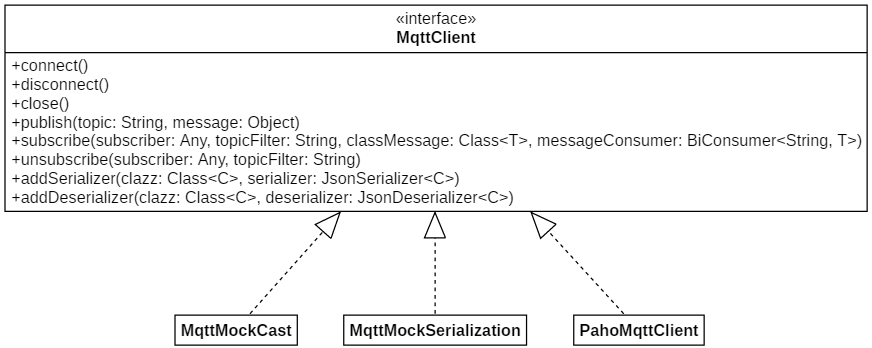
\includegraphics[width=\textwidth]{figures/mqttClient.png}
    \caption{\textit{MqttClient} interface and its available implementations.\-
    ..........}
    \label{fig:mqtt}
\end{figure}

\noindent The designed architecture is not valid only for this project, but it is reusable in different project, so it was decided to export it as external library. The library is actually available on github\footnote{\href{https://github.com/Placu95/MqttClientWrapper}{https://github.com/Placu95/MqttClientWrapper}} and a release on Maven Central Repository is planned shortly.

\subsubsection{Network server}
The network server is the entity appointed to regulate the communication between gateways and applications, but there isn't any specification that define which tasks have to perform and which is its architecture. 
Different providers propose different solution. 
The solution designed for the simulator is composed from an autonomous simulator entity and perform two tasks:
\begin{enumerate}
    \item filtering of duplicated message in communication from gateways to applications
    \item selection of the best gateway to deliver an application's message to a LoRa mote. 
    Default strategy to choose the gateway select the gateway that has received the last transmission from the LoRa mote with more transmission power, but it is possible to change it defining different strategies. 
\end{enumerate}
\autoref{fig:GtoA} presents the new communication schema from a gateways that receive a LoRa transmission and the application; while \autoref{fig:AtoG} presents the new communication schema from an application, that want to send a message to a LoRa mote, to the selected gateway that perform the LoRa transmission.
\begin{figure}[h]
    \centering
    \begin{subfigure}{.495\textwidth}
        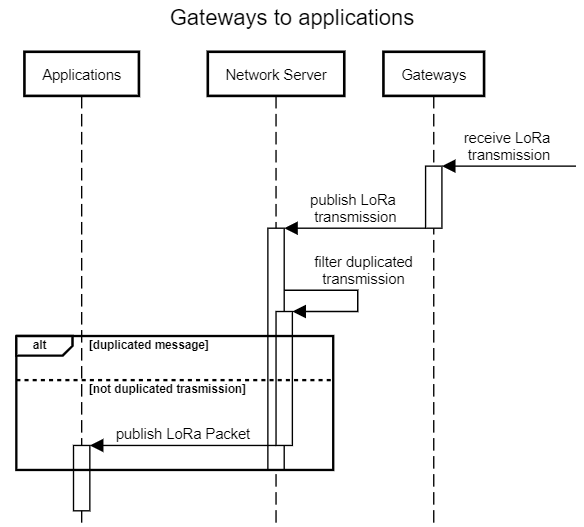
\includegraphics[scale=0.37]{figures/GtoApp.png}
        \caption{Communication from gateways \\to application}
        \label{fig:GtoA}
    \end{subfigure}
    \begin{subfigure}{.495\textwidth}
        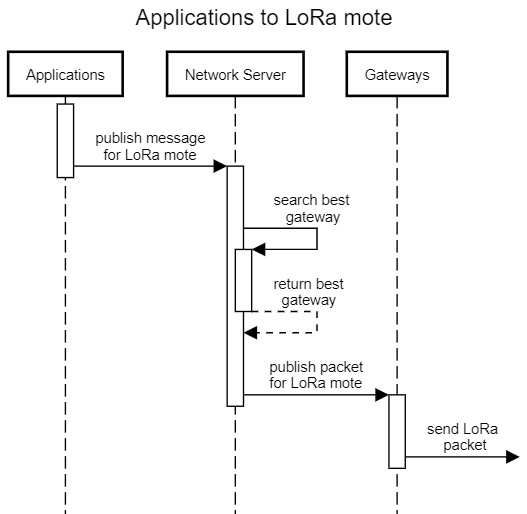
\includegraphics[scale=0.37]{figures/AppToG.png}
        \caption{Communication from application \\to gateways}
        \label{fig:AtoG}
    \end{subfigure}
    \caption{Communications between gateways and applications}
    \label{fig:netSer}
\end{figure}

\subsection{Timed run}
The simulator allows to execute two type of simulation: single run simulation and multiple run simulation, that consist simply in run more time a single run simulation. 
A single run simulation finish when all the mobile LoRa motes arrive to the respective destination. 
This behaviour is limiting because it is impossible execute simulation with only fixed LoRa mote or simulation that continue also after then every mote is arrived to destination. 
To go beyond these limitations it was introduced a new type of simulation: the \textit{Timed run} simulation. 
This type of simulation differs from the single run only for the condition of termination. 
The condition requires to define the duration of the simulation, so evaluate it as finished when is passed the defined time.

\subsection{Ranged sensor}
The DingNet simulator was developed to simulate self-adaptation applications based on received LoRa transmissions\todo{check ordine received}, so until now the real content of LoRa packet's payload was ignored.
The behaviour of different kinds of applications could instead depended from the payload. 
The idea is to define a new type of sensor that produces value in a configurable way splitting the region of simulation in a matrix of configurable dimension. 
So for each cell of the matrix define a list configurations. 
Each cell's configuration define the starting time of validity and the range for the value to produce. 
Then starting from this configuration will be produced a tricubic spline interpolation function where the three variable are: the two coordination of the matrix and the time; while the result is the corresponding sensor value.
Finally, when a mote require a new value to the the sensor, it produce the value considering the mote position and the simulation time.
The result is that each sensor inside the same cell will produce the same value at the same time. 
The architecture of this sensor is presented in \autoref{fig:rangedSensor}, where:
\begin{itemize}
    \item \textbf{SensorDataGenerator} $\rightarrow$ is basic interface for sensors, already present in the simulator
    \item \textbf{Cell} $\rightarrow$ is the representation of the cells that compose the configurable matrix
    \item \textbf{RangeValue} $\rightarrow$ is the range of validity for the value to produce
    \item \textbf{RangeDataGenerator} $\rightarrow$ is the abstract class that load the configuration file of the sensor, generate the interpolating function and produce values for LoRa motes. It require only to define the type of the two interfaces \textit{Cell} and \textit{RangeValue}.
\end{itemize}
% 
\begin{figure}[h]
    \centering
    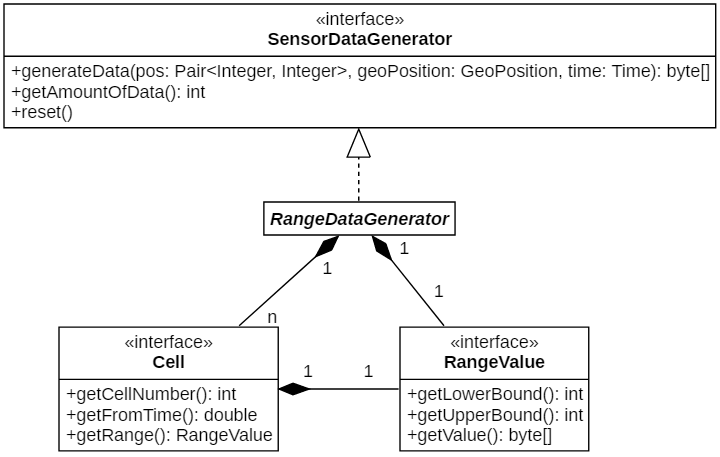
\includegraphics[scale=0.7]{figures/rangedSensor.png}
    \caption{Architecture of the configurable sensor}
    \label{fig:rangedSensor}
\end{figure}
% 
The actual file format for the sensor configuration file is \textit{toml}\footnote{\href{https://github.com/toml-lang/toml}{https://github.com/toml-lang/toml (Feb 2020)}}, but thanks to the \textit{konf}\footnote{\href{https://github.com/uchuhimo/konf}{https://github.com/uchuhimo/konf (Feb 2020)}} library (used to parse the file) it will be possible to change the file format with low effort.



\section{Aggregate programming over a LoRa-over-MQTT network}
\label{sec:contributionACOverDingNet}
This section presents the integration between the aggregate computing paradigm and a LoRa-over-MQTT like DingNet.
\todo{rifrasare prima frase?}
Firstly, to join these two concepts is necessary to define how map the networks entities in an aggregate computing system, and secondly identify potentially additional requirements or limitations for these entities.
In the aggregate computing viewpoint, a system is composed of a set of distributed heterogeneous computational entities, called nodes, that execute the same global program and communicate with a subset of them defined by a policy of neighbourhood. 
\todo{ci starebbe bene un while, ma poi sarebbero da unire le due frasi??}
The main entities that compose a LoRaWAN network are: LoRa motes, gateways, and network server; but at application level the only interesting entities are the LoRa motes.
So following the previous vision is natural mapping each LoRa mote in a node that represents its digital twin (from now called LoRa node) inside the aggregate system.
If LoRa nodes, on one hand, can be considered as generic nodes and do not require any specific neighbourhood's policy, or the use of particular communication technology to interact with their neighbours; at the other hand they have to support communication via MQTT. 
This requirement is necessary to enable bidirectional communication with the respective physical counterparts.
Finally, if on one hand they were identified the LoRa motes as the only entities of interest at the application level, on the other hand, it is necessary to analyse which network entities can host the aggregate nodes. 
% check se prima detto che posizione in cui eseguiamo i nodi non influisce il programma aggregato
In \cite{CCNCPS2018} the authors present a software architecture to enable the execution of aggregate computing programs on LoRa motes, but after evaluation of the proposed solution, they identify some issues due to the physical limitation of the technology communication. 
While these issues do not allow to execute aggregate computing program directly on the LoRa motes, they are not valid for the others network entities and does not exist any paper that identifies others possible issues.
Even if all the LoRaWAN network entities excluded the motes can host the aggregate node (LoRa nodes or others type of node), it is important to specify a limitation for the LoRa nodes. 
The LoRa nodes can interact with the respective LoRa mote only following the interaction schema defined from the LoRa-over-MQTT networks. 
For example, if a LoRa node is hosted by a LoRa gateway, that receives directly the transmissions of the respective LoRa mote, it cannot receive directly the packet, but it has to wait that is published on the MQTT broker.
The following subsection presents the software architecture designed to support the LoRa nodes inside an aggregate computing system defined in \textit{Protelis}. \todo{change defined - valutare se togliere ultima frase} \todo{add image?}
% disegnino con building block del sistema
% \begin{figure}[h]
%     \centering
%     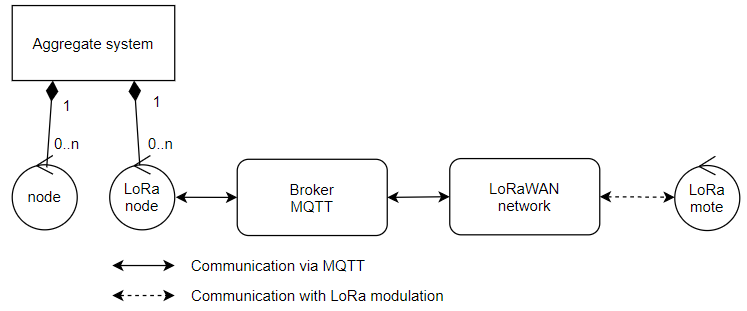
\includegraphics[width=\textwidth]{figures/ACplusLoRa.png}
%     \caption{Aggregate system with LoRa-over-MQTT network.}
%     \label{fig:ACplusLoRa}
% \end{figure}

\subsection{Integration of Protelis with DingNet}

The only things to do to enable developing of Protelis applications over the DingNet network is to satisfy the requirement previously identified.
\iffalse
The only requirement identified to support LoRa nodes inside an aggregate computing system is that they have to support MQTT communication. 
\fi
That requirement represents a specific capability of this type of nodes and Protelis defines a single place appointed to host device capabilities, the \mbox{\textit{ExecutionContext}}.
\autoref{fig:execContext} shows the model of the \mbox{\textit{ExecutionContext}} designed for LoRa nodes. 
\begin{figure}[H]
    \centering
    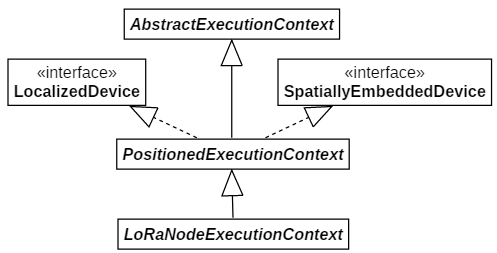
\includegraphics{figures/execContext.png}
    \caption{Model of \textit{ExecutionContext} for LoRa nodes}
    \label{fig:execContext}
\end{figure}
\noindent For devices spatially embedded and mainly used to transmit sensor values, their position is a relevant information, so it is defined\todo{bho} \mbox{\textit{PositionedExecutionContext}} that extends \mbox{\textit{AbstractExecutionContext}} (provided by Protelis) implementing the two interfaces that define functions to obtain spatial information of the device.
\iffalse
\mbox{\textit{LoRaNodeExecutionContext}} adds support for MQTT communication (satisfying the identified requirement), encapsulate the subscription to the MQTT topic to receive the sensed values by the respective LoRa mote, and manage the received packet adding the sensed values to the knowledge-based of the node or modifying the node position if the value belongs to the GPS sensor.
\fi
\mbox{\textit{LoRaNodeExecutionContext}} is the basic execution context for a LoRa node and it:\todo{check if}
% 
\begin{itemize}
    \item adds support for MQTT communication, satisfying the identified requirement
    \item encapsulates the subscription to the MQTT topic to receive the sensed values from the respective LoRa mote
    \item manages the received packet adding the sensed values to the knowledge-based of the node, or modifying its position if the value belongs to the GPS sensor.
\end{itemize}
% 
The designed model enables the design of Protelis application composed of LoRa nodes, but also not LoRa nodes, and an abstract model for these applications is reported in \autoref{fig:appP}. Protelis applications with this model are not only valid for the DingNet network but for all the LoRa-over-MQTT network that provide LoRa mote's data on a MQTT broker.
% 
\begin{figure}[H]
    \centering
    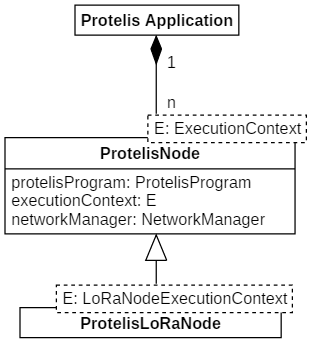
\includegraphics{figures/app.png}
    \caption{Abstract model of a Protelis application composed of LoRa nodes}
    \label{fig:appP}
\end{figure}
% 
\noindent To execute Protelis applications on the top of DingNet simulator, enabling the simulation of Protelis applications composed of LoRa nodes, is necessary one last small operation: unify the concept of time. 
This operation is necessary because the behaviour of every Protelis node depends also from the time in which the LoRa packets are received.
To do this it is sufficient wrapping the \mbox{\textit{LoRaNodeExecutionContext}} using the simulator time concept.


% \subsubsection{Support to mobility}
% Il resto è tutto un di più e per supportare mobilità, network-manager basato su mqtt, vicinato basato su distanza linea d'aria, aggiornamento vicinato ad ogni combiamento di posizione, 